% !TEX program = xelatex

\documentclass[10pt,a4paper]{article}
\usepackage[top = 1.5cm, bottom = 1.5cm, left = 1.5cm, right = 1.5cm]{geometry}

\usepackage{titling}
\usepackage[czech]{babel}
\usepackage{graphicx}
\usepackage{lmodern}
\usepackage{hyperref}
\usepackage{setspace}
\usepackage{csvsimple}
\usepackage{subcaption}

\usepackage{amsmath}
\usepackage{amssymb}
\usepackage{gensymb}
\usepackage{units}
\usepackage{bm}
\delimitershortfall=-1pt

\usepackage{gnuplottex}
\usepackage{epstopdf}

\usepackage{xltxtra}
\usepackage{xelatexemoji}

% no page break
\newenvironment{absolutelynopagebreak}
  {\par\nobreak\vfil\penalty0\vfilneg
   \vtop\bgroup}
  {\par\xdef\tpd{\the\prevdepth}\egroup
   \prevdepth=\tpd}


% redefine \sqrt
\usepackage{letltxmacro}
\makeatletter
\let\oldr@@t\r@@t
\def\r@@t#1#2{%
\setbox0=\hbox{$\oldr@@t#1{#2\,}$}\dimen0=\ht0
\advance\dimen0-0.2\ht0
\setbox2=\hbox{\vrule height\ht0 depth -\dimen0}%
{\box0\lower0.4pt\box2}}
\LetLtxMacro{\oldsqrt}{\sqrt}
\renewcommand*{\sqrt}[2][\ ]{\oldsqrt[#1]{#2\,}\,}
\makeatother

\def\ph{\phantom}
\def\vph{\vphantom}
\def\hph{\hphantom}

\newcommand{\comm}[2]{\left[ #1, #2 \right]}
\newcommand{\const}[1]{\text{\rmfamily\upshape #1}}
\newcommand{\norm}[1]{\left\lVert#1\right\rVert}

\newcommand{\mat}[1]{
    \begin{pmatrix}
        #1
    \end{pmatrix}
}

\newcommand{\mata}[2]{
    \left(
    \begin{array}{@{}#1@{}}
        #2
    \end{array}
    \right)
}

\renewcommand{\d}[1]{\;\const{d}#1}
\newcommand{\dd}[2]{\frac{\const{d} #1}{\const{d} #2} \;}
\newcommand{\pd}[2]{\frac{\partial  #1}{\partial  #2} \;}

\newcommand{\bra}[1]{\left< #1 \right|}
\newcommand{\ket}[1]{\left| #1 \right>}
\newcommand{\braket}[2]{\left< #1 \middle| #2 \right>}

\newcommand{\e}[1]{\const{e}^{#1}}
\renewcommand{\i}{\const{i}}

\newcommand{\Tr}{\operatorname{Tr}}

\begin{document}

\title{Matematika pro fyziky 1: The X-Files 👽️}
\author{Michal Grňo}
\date{\today}

\maketitle

\section{❓️❓️❓️}

\begin{gather*}
    \bm{p}, \bm{q} \in \mathbb{R}^2
    \;\;\;\;\;
    H = \norm{\bm{p}}^2 + \norm{\bm{q}}^2
    \\[10pt]
    \dot{q}_j = \pd{H}{p_j}
    \;\;\;\;\;
    \dot{p}_j = -\pd{H}{q_j} + (-1)^j \zeta \left( \pd{H}{p_1} - \pd{H}{p_2} \right)
\end{gather*}

\section{❗️❗️❗️}

\subsection{
    \texorpdfstring{
        $\pmb{ p,q = \mathit{?} }$
    }{
        p,q = ?
    }
}

\begin{align*}
    \bm{v} &= \mat{ \bm{q} \\ \bm{p} } = \mat{ q_1 \\ q_2 \\ p_1 \\ p_2}
    &
    \dot{\bm{v}} &= \mat{
        \pd{H}{p_1} \\ \pd{H}{p_2} \\
        -\pd{H}{q_1} - \zeta \left( \pd{H}{p_1} - \pd{H}{p_2} \right) \\
        -\pd{H}{q_2} + \zeta \left( \pd{H}{p_1} - \pd{H}{p_2} \right)
    }
    =
    \underbrace{
        2
        \mat{
            \ph{-}0 & \ph{-}0 & \ph{-}1 & \ph{-}0 \\
            \ph{-}0 & \ph{-}0 & \ph{-}0 & \ph{-}1 \\
            -1      & \ph{-}0 & -\zeta  & \ph{-}\zeta \\
            \ph{-}0 & -1      & \ph{-}\zeta & -\zeta
        }
    }_M \bm{v}
\end{align*}

\begin{align*}
    \boxed{
        \dot{\bm{v}} = M \bm{v} \;\;\;
        \implies \;\;\;
        \bm{v} = \exp(t M) \bm{v_0}, \;\;\;
        \bm{v_0} \in \mathbb{R}^2
    }
\end{align*}


\subsection{
    \texorpdfstring{
        $\pmb{ \exp(tM) = \mathit{?} }$
    }{
        exp(tM) = ?
    }
}
\begin{gather*}
    tM = P^{-1} \; J \; P
\end{gather*}
\begin{align*}
    \underbrace{
        2t
        \mat{
            \ph{-}0 & \ph{-}0 & \ph{-}1 & \ph{-}0 \\
            \ph{-}0 & \ph{-}0 & \ph{-}0 & \ph{-}1 \\
            -1      & \ph{-}0 & -\zeta  & \ph{-}\zeta \\
            \ph{-}0 & -1      & \ph{-}\zeta & -\zeta
        }
    }_{
        tM
    }
    =
    &\underbrace{
        \mat{\i & - \i & \frac{1}{\zeta + \sqrt{\zeta^{2} - 1}} & \frac{1}{\zeta - \sqrt{\zeta^{2} - 1}}\\\i & - \i & - \frac{1}{\zeta + \sqrt{\zeta^{2} - 1}} & \frac{1}{- \zeta + \sqrt{\zeta^{2} - 1}}\\1 & 1 & -1 & -1\\1 & 1 & 1 & 1}
    }_{
        P^{-1}
    }
    \\
    &\underbrace{
        \mat{- 2 \i t & 0 & 0 & 0\\0 & 2 \i t & 0 & 0\\0 & 0 & - 2 t \left(\zeta + \sqrt{\zeta^{2} - 1}\right) & 0\\0 & 0 & 0 & 2 t \left(- \zeta + \sqrt{\zeta^{2} - 1}\right)}
    }_{
        J
    }
    \\
    &\underbrace{
        \frac{1}{4}
        \mat{- \i & - \i & 1 & 1\\\i & \i & 1 & 1\\- \frac{1}{\sqrt{\zeta^{2} - 1}} & \frac{1}{\sqrt{\zeta^{2} - 1}} & - \frac{\zeta}{\sqrt{\zeta^{2} - 1}} - 1 & \frac{\zeta}{\sqrt{\zeta^{2} - 1}} + 1\\\frac{1}{\sqrt{\zeta^{2} - 1}} & - \frac{1}{\sqrt{\zeta^{2} - 1}} & \frac{\zeta}{\sqrt{\zeta^{2} - 1}} - 1 & - \frac{\zeta}{\sqrt{\zeta^{2} - 1}} + 1}
    }_{
        P
    }
\end{align*}
\begin{gather*}
    \\[25pt]
    \exp(tM) = \exp(P^{-1} J P) = P^{-1} \exp(J) P
    \\[15pt]
    \exp(tM) = P^{-1} \mat{
        e^{- 2 i t} & 0 & 0 & 0\\0 & e^{2 i t} & 0 & 0\\0 & 0 & e^{- 2 t \left(\zeta + \sqrt{\zeta^{2} - 1}\right)} & 0\\0 & 0 & 0 & e^{- 2 t \left(\zeta - \sqrt{\zeta^{2} - 1}\right)}
    } P
    \\[25pt]
\end{gather*}
\begin{gather*}
    \exp(tM) = \underbrace{\scalebox{0.25}{$\mat{\frac{e^{2 i t}}{4} + \frac{e^{- 2 i t}}{4} - \frac{e^{- 2 t \left(\zeta + \sqrt{\zeta^{2} - 1}\right)}}{4 \left(\zeta + \sqrt{\zeta^{2} - 1}\right) \sqrt{\zeta^{2} - 1}} + \frac{e^{- 2 t \left(\zeta - \sqrt{\zeta^{2} - 1}\right)}}{4 \left(\zeta - \sqrt{\zeta^{2} - 1}\right) \sqrt{\zeta^{2} - 1}} & \frac{e^{2 i t}}{4} + \frac{e^{- 2 i t}}{4} + \frac{e^{- 2 t \left(\zeta + \sqrt{\zeta^{2} - 1}\right)}}{4 \left(\zeta + \sqrt{\zeta^{2} - 1}\right) \sqrt{\zeta^{2} - 1}} - \frac{e^{- 2 t \left(\zeta - \sqrt{\zeta^{2} - 1}\right)}}{4 \left(\zeta - \sqrt{\zeta^{2} - 1}\right) \sqrt{\zeta^{2} - 1}} & \frac{\left(i \left(1 - \zeta^{2}\right) e^{4 t \left(\zeta + i\right)} - \sqrt{\zeta^{2} - 1} e^{2 t \left(\zeta - \sqrt{\zeta^{2} - 1} + i\right)} + \sqrt{\zeta^{2} - 1} e^{2 t \left(\zeta + \sqrt{\zeta^{2} - 1} + i\right)} + i \left(\zeta^{2} - 1\right) e^{4 t \zeta}\right) e^{- 2 t \left(2 \zeta + i\right)}}{4 \left(\zeta^{2} - 1\right)} & \frac{\left(i \left(1 - \zeta^{2}\right) e^{4 t \left(\zeta + i\right)} + \sqrt{\zeta^{2} - 1} e^{2 t \left(\zeta - \sqrt{\zeta^{2} - 1} + i\right)} - \sqrt{\zeta^{2} - 1} e^{2 t \left(\zeta + \sqrt{\zeta^{2} - 1} + i\right)} + i \left(\zeta^{2} - 1\right) e^{4 t \zeta}\right) e^{- 2 t \left(2 \zeta + i\right)}}{4 \left(\zeta^{2} - 1\right)}\\\frac{e^{2 i t}}{4} + \frac{e^{- 2 i t}}{4} + \frac{e^{- 2 t \left(\zeta + \sqrt{\zeta^{2} - 1}\right)}}{4 \left(\zeta + \sqrt{\zeta^{2} - 1}\right) \sqrt{\zeta^{2} - 1}} - \frac{e^{- 2 t \left(\zeta - \sqrt{\zeta^{2} - 1}\right)}}{4 \left(\zeta - \sqrt{\zeta^{2} - 1}\right) \sqrt{\zeta^{2} - 1}} & \frac{e^{2 i t}}{4} + \frac{e^{- 2 i t}}{4} - \frac{e^{- 2 t \left(\zeta + \sqrt{\zeta^{2} - 1}\right)}}{4 \left(\zeta + \sqrt{\zeta^{2} - 1}\right) \sqrt{\zeta^{2} - 1}} + \frac{e^{- 2 t \left(\zeta - \sqrt{\zeta^{2} - 1}\right)}}{4 \left(\zeta - \sqrt{\zeta^{2} - 1}\right) \sqrt{\zeta^{2} - 1}} & \frac{\left(i \left(1 - \zeta^{2}\right) e^{4 t \left(\zeta + i\right)} + \sqrt{\zeta^{2} - 1} e^{2 t \left(\zeta - \sqrt{\zeta^{2} - 1} + i\right)} - \sqrt{\zeta^{2} - 1} e^{2 t \left(\zeta + \sqrt{\zeta^{2} - 1} + i\right)} + i \left(\zeta^{2} - 1\right) e^{4 t \zeta}\right) e^{- 2 t \left(2 \zeta + i\right)}}{4 \left(\zeta^{2} - 1\right)} & \frac{\left(i \left(1 - \zeta^{2}\right) e^{4 t \left(\zeta + i\right)} - \sqrt{\zeta^{2} - 1} e^{2 t \left(\zeta - \sqrt{\zeta^{2} - 1} + i\right)} + \sqrt{\zeta^{2} - 1} e^{2 t \left(\zeta + \sqrt{\zeta^{2} - 1} + i\right)} + i \left(\zeta^{2} - 1\right) e^{4 t \zeta}\right) e^{- 2 t \left(2 \zeta + i\right)}}{4 \left(\zeta^{2} - 1\right)}\\\frac{\left(i \left(1 - \zeta^{2}\right) e^{4 t \zeta} + \sqrt{\zeta^{2} - 1} e^{2 t \left(\zeta - \sqrt{\zeta^{2} - 1} + i\right)} - \sqrt{\zeta^{2} - 1} e^{2 t \left(\zeta + \sqrt{\zeta^{2} - 1} + i\right)} + i \left(\zeta^{2} - 1\right) e^{4 t \left(\zeta + i\right)}\right) e^{- 2 t \left(2 \zeta + i\right)}}{4 \left(\zeta^{2} - 1\right)} & \frac{\left(i \left(1 - \zeta^{2}\right) e^{4 t \zeta} - \sqrt{\zeta^{2} - 1} e^{2 t \left(\zeta - \sqrt{\zeta^{2} - 1} + i\right)} + \sqrt{\zeta^{2} - 1} e^{2 t \left(\zeta + \sqrt{\zeta^{2} - 1} + i\right)} + i \left(\zeta^{2} - 1\right) e^{4 t \left(\zeta + i\right)}\right) e^{- 2 t \left(2 \zeta + i\right)}}{4 \left(\zeta^{2} - 1\right)} & \frac{\left(\left(- \zeta + \sqrt{\zeta^{2} - 1}\right) \sqrt{\zeta^{2} - 1} e^{2 t \left(\zeta + \sqrt{\zeta^{2} - 1} + i\right)} + \left(\zeta + \sqrt{\zeta^{2} - 1}\right) \sqrt{\zeta^{2} - 1} e^{2 t \left(\zeta - \sqrt{\zeta^{2} - 1} + i\right)} + \left(\zeta^{2} - 1\right) e^{4 t \zeta} + \left(\zeta^{2} - 1\right) e^{4 t \left(\zeta + i\right)}\right) e^{- 2 t \left(2 \zeta + i\right)}}{4 \left(\zeta^{2} - 1\right)} & \frac{\left(\left(\zeta - \sqrt{\zeta^{2} - 1}\right) \sqrt{\zeta^{2} - 1} e^{2 t \left(\zeta + \sqrt{\zeta^{2} - 1} + i\right)} - \left(\zeta + \sqrt{\zeta^{2} - 1}\right) \sqrt{\zeta^{2} - 1} e^{2 t \left(\zeta - \sqrt{\zeta^{2} - 1} + i\right)} + \left(\zeta^{2} - 1\right) e^{4 t \zeta} + \left(\zeta^{2} - 1\right) e^{4 t \left(\zeta + i\right)}\right) e^{- 2 t \left(2 \zeta + i\right)}}{4 \left(\zeta^{2} - 1\right)}\\\frac{\left(i \left(1 - \zeta^{2}\right) e^{4 t \zeta} - \sqrt{\zeta^{2} - 1} e^{2 t \left(\zeta - \sqrt{\zeta^{2} - 1} + i\right)} + \sqrt{\zeta^{2} - 1} e^{2 t \left(\zeta + \sqrt{\zeta^{2} - 1} + i\right)} + i \left(\zeta^{2} - 1\right) e^{4 t \left(\zeta + i\right)}\right) e^{- 2 t \left(2 \zeta + i\right)}}{4 \left(\zeta^{2} - 1\right)} & \frac{\left(i \left(1 - \zeta^{2}\right) e^{4 t \zeta} + \sqrt{\zeta^{2} - 1} e^{2 t \left(\zeta - \sqrt{\zeta^{2} - 1} + i\right)} - \sqrt{\zeta^{2} - 1} e^{2 t \left(\zeta + \sqrt{\zeta^{2} - 1} + i\right)} + i \left(\zeta^{2} - 1\right) e^{4 t \left(\zeta + i\right)}\right) e^{- 2 t \left(2 \zeta + i\right)}}{4 \left(\zeta^{2} - 1\right)} & \frac{\left(\left(\zeta - \sqrt{\zeta^{2} - 1}\right) \sqrt{\zeta^{2} - 1} e^{2 t \left(\zeta + \sqrt{\zeta^{2} - 1} + i\right)} - \left(\zeta + \sqrt{\zeta^{2} - 1}\right) \sqrt{\zeta^{2} - 1} e^{2 t \left(\zeta - \sqrt{\zeta^{2} - 1} + i\right)} + \left(\zeta^{2} - 1\right) e^{4 t \zeta} + \left(\zeta^{2} - 1\right) e^{4 t \left(\zeta + i\right)}\right) e^{- 2 t \left(2 \zeta + i\right)}}{4 \left(\zeta^{2} - 1\right)} & \frac{\left(\left(- \zeta + \sqrt{\zeta^{2} - 1}\right) \sqrt{\zeta^{2} - 1} e^{2 t \left(\zeta + \sqrt{\zeta^{2} - 1} + i\right)} + \left(\zeta + \sqrt{\zeta^{2} - 1}\right) \sqrt{\zeta^{2} - 1} e^{2 t \left(\zeta - \sqrt{\zeta^{2} - 1} + i\right)} + \left(\zeta^{2} - 1\right) e^{4 t \zeta} + \left(\zeta^{2} - 1\right) e^{4 t \left(\zeta + i\right)}\right) e^{- 2 t \left(2 \zeta + i\right)}}{4 \left(\zeta^{2} - 1\right)}}$}}_{😂️👌️}
    \\[25pt]
    \exp(tM) |_{\zeta=0} = \mat{\cos{\left(2 t \right)} & 0 & \sin{\left(2 t \right)} & 0\\0 & \cos{\left(2 t \right)} & 0 & \sin{\left(2 t \right)}\\- \sin{\left(2 t \right)} & 0 & \cos{\left(2 t \right)} & 0\\0 & - \sin{\left(2 t \right)} & 0 & \cos{\left(2 t \right)}}
    \\[25pt]
\end{gather*}

\subsection{
    \texorpdfstring{
        $\pmb{ \det\exp(tM) = \mathit{?} }$
    }{
        det exp(tM) = ?
    }
}
\begin{gather*}
    \det \exp(tM) = \exp \Tr(tM) =
    \exp\left( t \Tr(M) \right) =
    \exp\left( 2t \left(-2\zeta\right) \right) =
    \exp(-4t\zeta)
    \\[10pt]
    \zeta = 0 \;\;\; \implies \;\;\;
    \det\exp(tM) = 1 \;\;\; \implies \;\;\;\
    \dd{}{t}
    \iiiint_{\Omega(t)}
    \d{q_1} \d{q_2} \d{p_1} \d{p_2} = 0
    \\[10pt]
    \zeta \neq 0 \;\;\; \implies \;\;\;
    \iiiint_{\Omega(t)}
    \d{q_1} \d{q_2} \d{p_1} \d{p_2}
    =
    \e{-4 t \zeta}
    \iiiint_{\Omega(0)}
    \d{q_1} \d{q_2} \d{p_1} \d{p_2}
\end{gather*}


\subsection{
    \texorpdfstring{
        $\pmb{ p(t)|_{\zeta=0}, \; q(t)|_{\zeta=0} = \mathit{?} }$
    }{
        p(t)|\{z=0\}, q(t)|\{z=0\} = ?
    }
}
\begin{gather*}
    \mat{
        \bm{q}|_{\zeta=0} \\ \bm{p}|_{\zeta=0}
    }
    =
    \exp(tM)
    \mat{
        \bm{q_0} \\ \bm{p_0}
    }
    \\[5pt]
\end{gather*}
\begin{gather*}
    \left.
    \mat{
        q_1(t) \\ q_2(t) \\ p_1(t) \\ p_2(t)
    }
    \right|_{\zeta=0}
    =
    \mat{\cos{\left(2 t \right)} & 0 & \sin{\left(2 t \right)} & 0\\0 & \cos{\left(2 t \right)} & 0 & \sin{\left(2 t \right)}\\- \sin{\left(2 t \right)} & 0 & \cos{\left(2 t \right)} & 0\\0 & - \sin{\left(2 t \right)} & 0 & \cos{\left(2 t \right)}}
    \mat{
        q_{10} \\ q_{20} \\ p_{10} \\ p_{20}
    }
    \\[5pt]
\end{gather*}
\begin{gather*}
    \\
    q_1(t)|_{\zeta=0} = p_{10} \sin{\left(2 t \right)} + q_{10} \cos{\left(2 t \right)}
    \\[5pt]
    q_2(t)|_{\zeta=0} = p_{20} \sin{\left(2 t \right)} + q_{20} \cos{\left(2 t \right)}
    \\[5pt]
    p_1(t)|_{\zeta=0} = p_{10} \cos{\left(2 t \right)} - q_{10} \sin{\left(2 t \right)}
    \\[5pt]
    p_2(t)|_{\zeta=0} = p_{20} \cos{\left(2 t \right)} - q_{20} \sin{\left(2 t \right)}
    \\[10pt]
\end{gather*}

\begin{figure}
    \centering
    \begin{subfigure}{.3\textwidth}
        \centering
        \begin{gnuplot}[terminal=epslatex,terminaloptions={color size 5cm, 5cm}]
            set macros
            set parametric
            set trange [0:pi]

            set key left top
            set xlabel '$q_1$'
            set ylabel '$q_2$'
            set title '$\zeta = 0$'

            set xrange [-1.5:1.5]
            set yrange [-1.5:1.5]

            set lmargin at screen 0
            set bmargin at screen 0
            set rmargin at screen 1
            set tmargin at screen 1
            unset xtics
            unset ytics

            q1(q10,q20,p10,p20,t) = p10*sin(2*t) + q10*cos(2*t)
            q2(q10,q20,p10,p20,t) = p20*sin(2*t) + q20*cos(2*t)

            comb = \
                '1,1,1,1  1,1,0,1  1,0,1,1  0,1,1,1  1,1,0,0   1,0,1,0  0,1,1,0  1,0,0,1  0,1,0,1  0,0,1,1'
            macro = ''
            do for [i=1:words(comb)] {
                w = word(comb,i)
                if (!(macro eq '')) { macro = macro . ', '}
                macro = macro . 'q1('.w.',t), q2('.w.',t) not'
            }

            plot @macro
        \end{gnuplot}
    \end{subfigure}%
    \begin{subfigure}{.3\textwidth}
        \centering
        \begin{gnuplot}[terminal=epslatex,terminaloptions={color size 5cm, 5cm}]
            set macros

            set key left top
            set xlabel '$q_1$'
            set title '$\zeta = 0.2$'

            set xrange [-1.5:1.5]
            set yrange [-1.5:1.5]

            set lmargin at screen 0
            set bmargin at screen 0
            set rmargin at screen 1
            set tmargin at screen 1
            unset xtics
            unset ytics

            comb = \
                '1,1,1,1  1,1,0,1  1,0,1,1  0,1,1,1  1,1,0,0   1,0,1,0  0,1,1,0  1,0,0,1  0,1,0,1  0,0,1,1'
            macro = ''
            do for [i=1:words(comb)] {
                w = word(comb,i)
                if (!(macro eq '')) { macro = macro . ', '}
                macro = macro . '"xfiles_z02_'.w.'.dat" w l not'
            }

            plot @macro
        \end{gnuplot}
    \end{subfigure}
    \begin{subfigure}{.3\textwidth}
        \centering
        \begin{gnuplot}[terminal=epslatex,terminaloptions={color size 5cm, 5cm}]
            set macros

            set key left top
            set xlabel '$q_1$'
            set title '$\zeta = 0.5$'

            set xrange [-1.5:1.5]
            set yrange [-1.5:1.5]

            set lmargin at screen 0
            set bmargin at screen 0
            set rmargin at screen 1
            set tmargin at screen 1
            unset xtics
            unset ytics
  
            comb = \
                '1,1,1,1  1,1,0,1  1,0,1,1  0,1,1,1  1,1,0,0   1,0,1,0  0,1,1,0  1,0,0,1  0,1,0,1  0,0,1,1'
            macro = ''
            do for [i=1:words(comb)] {
                w = word(comb,i)
                if (!(macro eq '')) { macro = macro . ', '}
                macro = macro . '"xfiles_z05_'.w.'.dat" w l not'
            }
    
            plot @macro
        \end{gnuplot}
      \end{subfigure}
\end{figure}

\subsection{
    \texorpdfstring{
        $\pmb{ \mathit{Michal Gr\check{n}o} = \mathit{?} }$
    }{
        Michal Grňo = ?
    }
}
\centering
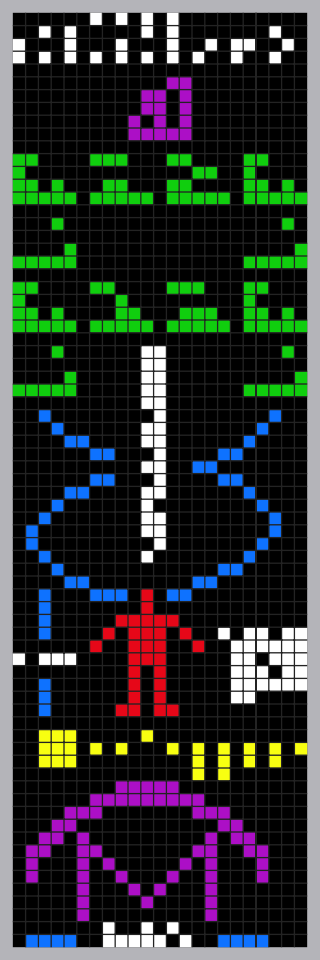
\includegraphics[height=15cm,keepaspectratio]{arecibo.png}


\end{document}
